\pagestyle{empty}
\chapter*{\centering \large DAFTAR RIWAYAT HIDUP}
\thispagestyle{empty}

\begin{wrapfigure}{l}{4cm}
	\vspace{-25pt}
	\begin{center}
		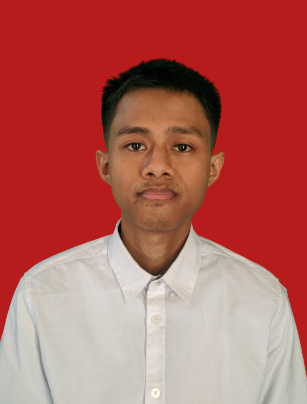
\includegraphics[width=0.27\textwidth]{gambar/pas-foto}
	\end{center}
	\vspace{-80pt}
\end{wrapfigure}

\noindent \textbf{MUHAMAD RIZKI.}  Lahir di Bogor, 27 Juli 1998.  Anak pertama dari pasangan Bapak Achmad Jamiat (alm) dan Ibu Kartinah. Saat ini beralamatkan di Jl. Masjid Al-Ittihad no. 06 RT 10 RW 05 kel. Bojong Pondok Terong kec. Cipayung, Kota Depok.

\vspace{0.5cm}
\noindent
\begin{center}
	\begin{flushright}
		\begin{tabular}{lcl}
			No. Ponsel	& :&  082295121172 \\
			Email	& :&  muhamadrizki109@gmail.com
		\end{tabular}
	\end{flushright}
\end{center}
\vspace{0.5cm}

\noindent \textbf{Riwayat Pendidikan} : Penulis mengawali pendidikan di MI Arrahmaniyyah Depok pada tahun 2004 - 2010. Setelah itu, penulis melanjutkan studi ke SMPN 9 Depok hingga tahun 2013. Kemudian melanjutkan ke SMAN 9 Bogor hingga tahun 2016. Di Tahun 2016 penulis melanjutkan ke Universitas Negeri Jakarta (UNJ), Program Studi Ilmu Komputer, melalui jalur SNMPTN dengan beasiswa BIDIKMISI dan kemudian lulus di tahun 2022.
%Di pertengahan tahun 2022 (Senin, 18 Februari 2019) penulis telah memperoleh gelar Sarjana Komputer (S.Kom), Program Studi Ilmu Komputer, Fakultas Matematika dan Ilmu Pengetahuan Alam, Universitas Negeri Jakarta.

\noindent \textbf{Riwayat Organisasi} : Selama di bangku perkuliahan, penulis tergabung dengan organisasi kemahasiswaan lain seperti, Masjid Ulul Albaab sebagai staff Syiar periode 2017.  Penulis juga berpartisipasi dalam organisasi keilmiahan di Program Studi Ilmu Komputer yaitu DEFAULT, dimana penulis tergabung sebagai anggota divisi \textit{web}. Penulis juga kerap mengikuti kepanitiaan kegiatan yang diadakan oleh lembaga dakwah fakultas (MUA), dan komunitas/\textit{underbow} lembaga (Default). 

\noindent \textbf{Tentang Skripsi} : Skripsi ini merupakan karya terbaik penulis yang diberikan untuk civitas akademika Universitas Negeri Jakarta. Besar harapan penulis agar skripsi ini dapat bermanfaat bagi semua yang membaca dan menggunakan hasil penelitian ini. Saran dan masukan mengenai skripsi ini dapat disampaikan melalui email muhamadrizki109@gmail.com